% !TEX TS-program = pdflatex
% !TEX encoding = UTF-8 Unicode

% This is a simple template for a LaTeX document using the "article" class.
% See "book", "report", "letter" for other types of document.

\documentclass[11pt]{article} % use larger type; default would be 10pt

\usepackage[utf8]{inputenc} % set input encoding (not needed with XeLaTeX)

%%% Examples of Article customizations
% These packages are optional, depending whether you want the features they provide.
% See the LaTeX Companion or other references for full information.

%%% PAGE DIMENSIONS
\usepackage{geometry} % to change the page dimensions
\geometry{a4paper} % or letterpaper (US) or a5paper or....
% \geometry{margin=2in} % for example, change the margins to 2 inches all round
% \geometry{landscape} % set up the page for landscape
%   read geometry.pdf for detailed page layout information

\usepackage{graphicx} % support the \includegraphics command and options

% \usepackage[parfill]{parskip} % Activate to begin paragraphs with an empty line rather than an indent

%%% PACKAGES
\usepackage{booktabs} % for much better looking tables
\usepackage{array} % for better arrays (eg matrices) in maths
\usepackage{paralist} % very flexible & customisable lists (eg. enumerate/itemize, etc.)
\usepackage{verbatim} % adds environment for commenting out blocks of text & for better verbatim
\usepackage{subfig} % make it possible to include more than one captioned figure/table in a single float
% These packages are all incorporated in the memoir class to one degree or another...

%%% HEADERS & FOOTERS
\usepackage{fancyhdr} % This should be set AFTER setting up the page geometry
\pagestyle{fancy} % options: empty , plain , fancy
\renewcommand{\headrulewidth}{0pt} % customise the layout...
\lhead{}\chead{}\rhead{}
\lfoot{}\cfoot{\thepage}\rfoot{}

%%% SECTION TITLE APPEARANCE
\usepackage{sectsty}


\allsectionsfont{\sffamily\mdseries\upshape} % (See the fntguide.pdf for font help)
% (This matches ConTeXt defaults)

%%% ToC (table of contents) APPEARANCE
\usepackage[nottoc,notlof,notlot]{tocbibind} % Put the bibliography in the ToC
\usepackage[titles,subfigure]{tocloft} % Alter the style of the Table of Contents
\renewcommand{\cftsecfont}{\rmfamily\mdseries\upshape}
\renewcommand{\cftsecpagefont}{\rmfamily\mdseries\upshape} % No bold!

%%% END Article customizations


\usepackage[bulgarian]{babel}
\usepackage{physics}
\usepackage{amsmath}
\usepackage{centernot}
\usepackage{url}
\usepackage{graphicx}
\graphicspath{ {.} }
\usepackage{amsfonts}
\usepackage{xcolor}
\usepackage{enumitem}
\usepackage{systeme}
\usepackage{listings}
\usepackage[cache=false]{minted}



%%% The "real" document content comes below...

\title{13. Структури от данни и алгоритми. Анализ на алгоритми. Абстрактни типове от данни}
\author{Play4u}
%\date{} % Activate to display a given date or no date (if empty),
         % otherwise the current date is printed
         

\newcommand{\lrangle}[1]{\left\langle #1 \right\rangle}

\newcommand{\oversetModels}[1]{\overset{#1}{\models}}

\newcommand{\italicBold}[1]{\textbf{\emph{#1}}}

\newcommand{\definition}{\italicBold{Дефиниция: }}
\newcommand{\theorem}{\italicBold{Теорема: }}
\newcommand{\lemma}{\italicBold{Лема: }}
\newcommand{\proof}{\italicBold{Доказателство: }}
\newcommand{\statement}{\italicBold{Твърдение: }}
\newcommand{\source}{\italicBold{Източник: }}

\newcommand{\integral}[4]{\displaystyle \int_{#1}^{#2}#3\,#4}

\newcommand{\redText}[1]{\textcolor{red}{#1}}

\newcommand{\curlies}[1]{\{#1\}}
\newcommand{\overbar}[1]{\mkern 1.5mu\overline{\mkern-1.5mu#1\mkern-1.5mu}\mkern 1.5mu}

\newcommand{\enumNum}{\renewcommand{\theenumi}{\arabic{enumi}}}
\newcommand{\enumlet}{\renewcommand{\theenumi}{\alph{enumi}}} 

\begin{document}
\maketitle

\italicBold{Конспект: } Изложението на въпроса трябва да включва следните по-съществени елементи:

\enumNum
\begin{enumerate}[noitemsep]
	\item Основи на анализа на алгоритми: Асимптотична нотация на сложността. Основни рекурентни формули. Примери за анализ на алгоритми.
	\item Абстрактни типове от данни. Интерфейс и реализиция.
	\item Свързани спиъсци. Обработка на списъци.
	\item Структура от данни стек. Реализация.
	\item Структура от данни опашка. Реализация.
	\item Дървета. Типове дървета.
	\item Сортиране. Елементарни методи за сортиране.
	\item Сортиране. Quicksort.\\\par
\end{enumerate}

\section{Основи на анализа на алгоритми}
Един алгоритъм е интересен (от гледна точка на математиката) в няколко аспекта:

\begin{itemize}[noitemsep]
	\item коректност - т.е дали решава зададената задача.
	\item времева сложност - т.е за колко стъпки ще завърши изпълнението си. Обърнете внимание, че алгоритмите работят винаги за някакъв цяло число брой стъпки което може да бъде измерено
	\item пространствена сложност - колко памет заемат, докато завършат.
\end{itemize}

Ние ще описваме измерването на слжоността на алгоритъма спрямо време и памет. Нека вземем за пример измерването на сложността по време, т.е. колко операции извършва алгоритъма до неговото завършване. Можем да го измерим по няколко начина:
\begin{itemize}[noitemsep]
	\item в най-лошия случай (worst-case) - т.е от всички входни данни в дадена група изчислим коя точно входна данна кара алгоритъма да извърши най-много стъпки.
	\item средна стойност (average) - т.е ако вземем всички входни данни в дадена група, изчислим за колко време работи алгоритъмът над тях, и вземем средното аритметично на всичко това, ще получим средната стойност

\end{itemize} 

\subsection{Асимптоматичен анализ}
Когато анализираме поведението на дадена функция (например времева сложност), доста по-удачно е вместо да се стремим да намерим точния вид на функцията, който примерно изглежда така: $T(n) = 12 n^2 + 94 n + 30940$ да се задоволим просто с $n^{2}$. Причината заради това е, че науката(и практиката) е показала , че при достатъчно голямо $N$ някои функции доминират други(стават безкрайно по-значими). Пр.: \\
\centerline{Нека: $T(n) = n^2 + 94 n$}
Ако $N$ клони към безкрайност $n^2$ отговаря за ~100\% от цялото време за изпълнение на алгоритъма. Така, сега ще покажем как можем да докажем, че горната стойност всъщност има сложност, която е равна на $n^2$. 

Нека дефинираме следното множество от функции\\
\begin{align} \Theta(g(n)) = \{ f(n) | \exists c_1, c_2 \in \mathbb R_+\ \exists n_0 \in \mathbb N : \forall n \ge n_0 \quad 0 \le c_1 g(n) \le f(n) \le c_2 g(n) \} \end{align}\\
Тита от $g(n)$ е равно на множеството от всички функции, за които съществуват две константи такива, че за достатъчно големи $N$ всяка стойност на $N$, $f(n)$ е в интервала $[c_1 g(n) : c_2 g(n)]$. Ще записваме $T(n) = \Theta(n^2)$.\\\par

\definition (Горна граница - O) Всички функции, които са толкова бавни или по-бързи от $g(n)$:
\begin{align} O(g(n)) = \{ f(n) | \exists c > 0\ \exists n_0 > 0 : \forall n \ge n_0 \quad 0 \le f(n) \le cg(n) \} \end{align}

\definition (Долна граница - $\omega$) Всички толкова бавни или по-бавни:
\begin{align} \Omega(g(n)) = \{ f(n) | \exists c > 0\ \exists n_0 > 0 : \forall n \ge n_0 \quad 0 \le cg(n) \le f(n) \} \end{align}

\section{Абстрактни типове от данни}

\definition \textbf{(Абстрактни типове данни: )}Абстрактните типове данни са типовете(или класовете) на обекти, чиито поведение е дефинирано от множество от стойности, които могат да съдържат и множество операции, които могат да се извършват върху тях. Важното в тази дефиниция, е че тя единствено споменава за това какви операции могат да се извършват над множеството данни, но не и как тези операции ще бъдат имплементирани. Не се споменава как данните ще бъдат представени в паметта, нито какви алгоритми ще се използват за имплементацията на операциите. Затова и се наричат абстрактни - предоставят начини за работа с данните, който е независим от имплементацията.

\subsection{Свързани списъци}
Списъкът е крайна редица от елементи от един и същ тип. Операциите включване и изключване на елемент са допустими
на произволно място в редицата. Възможен е достъп до всеки елемент на редицата (пряк или непряк в зависимост от
реализацията на списъка).\par
Има два основни начина за представяне на списък в паметта на компютъра: свързано представяне с една връзка, свързано
представяне с две връзки и последователно представяне.\par
При свързаното представяне с една връзка последователните елементи на списъка се съхраняват на различни места в
оперативната памет, а не в последователно разположени полета. Връзката между отделните елементи се осъществява чрез
указател към следващия елемент. Ако елементът е последен в списъка, стойността на този указател трябва да бъде някаква
различима стойност (например NULL). За задаване на списъка е достатъчен указател към неговото начало. За удобство при
реализирането на операциите включване, изключване и обхождане се въвеждат още указатели към края и към текущ
елемент на списъка. В общия случай елементите на списъка при свързаното представяне с една връзка се състоят от две
полета – inf (данните, записани в елемента) и link (указател към следващия елемент).
При свързаното представяне с две връзки последователните елементи на списъка се съхраняват на различни места в
оперативната памет, а не в последователно разположени полета. Връзките между отделните елементи се осъществяват чрез
два указателя към следващия и към предхождащия елемент. Ако елементът е последен в списъка, стойността на указателя
към следващия елемент трябва да бъде някаква различима стойност (например NULL), аналогично за указателя към
предхождащия елемент за елемента в началото на списъка. За задаване на списъка е достатъчен указател към неговото
начало. За удобство при реализирането на операциите включване, изключване и обхождане се въвеждат още указатели към
края и указател към текущ елемент на списъка. В общия случай елементите на списъка при свързаното представяне с две
връзки се състоят от три полета – inf (данните, записани в елемента), next (указател към следващия елемент) и prev
(указател към предхождащия елемент).\\

За да покажем работата с един списък, ще покажем възможния интерфейс на един списък. За целта обаче, първо ще дефинираме структурата Item<T>, чрез която се представят елементите на списъка. За по-голяма общност, дефинираме структурата Item и класа LList като шаблони(тъй като ще използваме C++)

\begin{minted}{c++}
template<class T> struct Item {
	T inf;
	Item *link;
};
\end{minted} 

А сега и интерфейсът на нашия свързван списък.
\begin{minted}{c++}
template <class T> class LList {
public:
	LList(const T&);
	LList();
	~LList();
	LList(const LList &);
	LList& operator= (const LList&);
	void restartIterator (Item <T>* = NULL); //Връща итериращия обект в началото(главата на списъка)
	Item <T>* Iter(); //Връща текущият елемент, към който сочи итератора и го премества  една стъпка напред  
	bool IterView(T&) const; //Връща истина/лъжа дали има още елементи за итерация
	void InsertToEnd (const T&); //Вкарва елемент в края на списъка
	void InsertToBegin (const T&); //Вкарва елемент в началото на списъка
	void InsertAfter (Item <T>*, const T&); //Вкарва елемент след друг даден елемент
	void InsertBefore (Item <T>*, const T&); //Вкарва елемент преди друг даден елемент
	void DeleteAfter (Item <T>*, T&); //Изтрива елемент след друг даден елемент и записва информацията от изтрития такъв във втория аргумент
	void DeleteBefore (Item <T>*, T&); //Изтрива елемент преди друг даден елемент записва информацията от изтрития такъв във втория аргумент
	void DeleteElement (Item <T>*, T&); //Изтрива дадения елемент записва информацията от изтрития такъв във втория аргумент
	int length() const; //Връща броя елементи в списъка
	void print() const; //Удобна функция, за изкарване на съдържанието на списъка върху std::out в някакъв формат
	void concat (const LList&); //Конкатенира два списъка
	void reverse(); //Обръща реда на текущия списък
	bool isEmpty() const; //Връща истина/лъжа спрямо това дали списъка е празен
};
\end{minted}

\subsection{Стек}
Стекът е линейна динамична структура от данни. Стекът е крайна редица от елементи от един и същи тип. Операциите включване и изключване на елемент са допустими само за единия край на редицата, който се нарича връх на стека. Възможен е пряк достъп само до елемента, който се намира във върха на стека. При тази организация на логическите операции, последният включен елемент се изключва пръв. Затова стекът се определя още като структура “последен влязъл – пръв излязъл” (last in – first out, LIFO).
Широко се използват два основни начина за представяне на стек: последователно и свързвано. При последователното представяне, предварително в паметта се запазва блок, вътре в който се помества стекът и той там расте и се съкращава. При включване на елементи в стека, те се поместват в последователни адреси в неизползваната част веднага след върха на стека.
При свързаното представяне последователните елементи се съхраняват на различни места в оперативната памет, а не в последователно разположени полета. Връзката между отделните елементи се осъществява чрез указател към следващия елемент. Ако елементът е последен в стека, стойността на този указател трябва да бъде някаква различима стойност (например NULL). За задаване на стека е достатъчен указател към върха на стека. В общия случай елементите на стека при свързаното представяне се състоят от две полета – inf (данните, записани в елемента) и link (указател към следващия елемент). Сега ще дефинираме клас, който реализира свързаното представяне на стек.
Първо ще дефинираме помощен клас Item, който реализира двойната кутия, чрез която се представят елементите на стека.
За по-голяма общност, дефинираме класовете като шаблони.

\begin{minted}{c++}
template <class T> class Stack;
template <class T> class Item {
	friend class Stack <T>;
	private:
		Item (const T& x = 0) { 
			inf = x;
			link = NULL;
		}
		T inf;
		Item *link;
};
\end{minted}

Тъй като класът Item използва класът Stack в декларацията си, затова прототипът на класа Stack предшества декларацията на класа Item. Всички членове на Item са капсулирани. Чрез декларацията за приятелство, класът Item позволява само на класа Stack да създава и обработва негови обекти. Сега вече сме готови да дефинираме класът Stack. Тъй като стекът се реализира в динамичната памет, за този клас трябва изрично да се реализира каноничното представяне – деструктор, обикновени конструктори, конструктор за присвояване и операторна функция за присвояване.

\begin{minted}{c++}
template <class T> 
class Stack {
	public:
		Stack (const T&);
		Stack ();
		~Stack ();
		Stack (const Stack &);
		Stack& operator= (const Stack &);
		void push (const T&);
		bool pop (T&);
		bool top(T&) const;
		bool empty () const;
	private:
		Item<T> *start;
		void delStack();
		void copyStack (const Stack &);
	};
	template <class T> Stack<T>::Stack (const T& x){ 
		start = new Item<T> (x); 
	}
	template <class T> Stack<T>::Stack () { 
		start = NULL; 
	}
	template <class T> Stack<T>::~Stack (){ 
		delStack(); 
	}
	template <class T> Stack<T>::Stack (const Stack<T> &r){ 
		copyStack(r); 
	}
	template <class T> Stack<T>& operator= (const Stack<T> &r){ 
		if (this != &r) {
			delStack ();
			copyStack (r);
		}
		return *this;
	}
	template <class T> void Stack<T>::delStack () {
		Item<T> *p;
		while (start){ 
			p = start;
			start = start -> link;
			delete p;
		}
	}

	template <class T> void Stack<T>::copyStack (const Stack<T> &r){ 
		if (!r.start) start = NULL;
		else {
			Item<T> *p = r.start, *q, *s;
			start = new Item<T>(p -> inf);
			q = start;
			p = p -> link;
			while (p) { 
				s = new Item<T> (p -> inf);
				q -> link = s;
				q = s;
				p = p -> link;
			}
		}
	}



	template <class T> void Stack<T>::push (const T& x){ 
		Item<T> *p = new Item<T>(x);
		p -> link = start;
		start = p;
	}
	template <class T> bool Stack<T>::pop (T& x){ 
		if (!start) return false;
		Item<T> *p = start;
		x = start -> inf;
		start = start -> link;
		delete p;
		return true;
	}
	template <class T> bool Stack<T>::top (T& x) const{ 
		if (!start) return false;
		x = start -> inf; 
		return true;
	}
	template <class T> bool Stack<T>::empty () const { 
		return start == NULL; 
	}
};
\end{minted}

\subsection{Опашка}
Опашката е крайна редица от елементи от един и същи тип. Операцията включване е допустима за елементите от единия край на редицата, който се нарича край на опашката, а операцията изключване на елемент – само за елементите от другия край на редицата, който се нарича начало на опашката. Възможен е пряк достъп само до елемента, намиращ се в началото на опашката. При тази организация на логическите операции, пръв се изключва най-отдавна включеният елемент. Затова опашката се определя още като структура от данни  “пръв влязъл – пръв излязъл” (first in – first out, FIFO).
Широко се използват два основни начина за физическо представяне на опашка: последователно и свързано.
При последователното представяне първоначално в паметта се запазва блок, вътре в който опашката да расте и да се съкращава. Включването на елемент в опашката се осъществява чрез поместването му в последователни адреси в неизползваната част веднага след края на опашката. Обикновено се счита, че блокът от памет е цикличен – когато краят на опашката достигне края на разпределения блок памет, но има освободена памет в неговото начало, там може да се извърши включване на елементи.
При свързаното представяне последователните елементи на опашката се съхраняват на различни места в оперативната памет, а не в последователно разположени полета. Връзката между отделните елементи се осъществява чрез указател към следващия елемент. Ако елементът е последен в опашката, стойността на този указател трябва да бъде някаква различима стойност (например NULL). За задаване на опашката са достатъчни указатели към началото и края на опашката. В общия случай елементите на опашката при свързаното представяне се състоят от две полета – inf (данните, записани в елемента) и link (указател към следващия елемент). Сега ще дефинираме клас, който реализира свързаното представяне на опашка.
Първо ще дефинираме помощен клас Item, който реализира двойната кутия, чрез която се представят елементите на опашката.
За по-голяма общност, дефинираме класовете като шаблони.

\begin{minted}{c++}
template <class T> class Queue;
template <class T> class Item {
friend class Queue <T>;
private:
	Item (const T& x = 0){ 
		inf = x;
		link = NULL;
	}
	T inf;
	Item *link;
};
\end{minted}
Тъй като класът Item използва класът Queue в декларацията си, затова прототипът на класа Queue предшества декларацията на класа Item. Всички членове на Item са капсулирани. Чрез декларацията за приятелство, класът Item позволява само на класа Queue да създава и обработва негови обекти. Сега вече сме готови да дефинираме класът Queue. Тъй като опашката се реализира в динамичната памет, за този клас трябва изрично да се реализира каноничното представяне – деструктор, обикновени конструктори, конструктор за присвояване и операторна функция за присвояване.


\begin{minted}{c++}
template <class T> class Queue {
	public:
		Queue(const T&);
		Queue();
		~Queue();
		Queue (const Queue &);
		Queue& operator= (const Queue &) ;
		void InsertElem (const T&);
		bool DeleteElem (T &);
		bool ViewElem(T &) const;
		bool empty() const;
	private:
		Item<T> *front, *rear;
		void delQueue();
		void copyQueue (const Queue &);
	} ;
	template <class T> Queue<T>::Queue(const T& x){ 
		front = new Item<T>(x);
		rear = front;
	}
	template <class T> Queue<T>::Queue() {
		front = rear = NULL;
	}
	template <class T> Queue<T>::~Queue() {
		 delQueue();
	}	
	template <class T> Queue<T>::Queue (const Queue<T> &r){ 
		copyQueue (r); 
	}
	template <class T> Queue<T>& Queue<T>::operator= (const Queue<T> &r){ 
		if (this != &r){ 
			delQueue();
			copyQueue(r);	
		}
		return *this;
	}
	template <class T> void Queue<T>::delQueue() { 
		T x;
		while (DeleteElem(x));
	}
	template <class T> void Queue<T>::copyQueue(const Queue<T> &r) { 
		front = rear = NULL;
		 if (r.front) {
			Item <T> *p = r.front;
			while (p) { 
				InsertElem (p -> inf);
				p = p -> link;
			}
		}
	}
	template <class T> void Queue<T>::InsertElem (const T& x){ 
		Item <T> *p = new Item<T>(x);
		if (front) { rear->link = p; rear = p; }
		else front = rear = p;
	}
	template <class T> bool Queue<T>::DeleteElem (T &x){ 
		if (!front) return false;
		Item <T> *p = front;
		x = p -> inf;
		if (front == rear) front = rear = NULL;
		else front = front -> link;
		delete p;
		return true;}
	template <class T> bool Queue<T>::ViewElem(T &x) const { 
		if (!front) return false;
		x = front -> inf;
		return true;
	}
	template <class T> bool Queue<T>::empty() const{ 
	return front == NULL; 
	}
\end{minted}

\textit{\textbf{Последователна (статична) реализация на стек и опашка}}\\
Важно е да отбележим, че съществува още един начин за реализация на гореспоменатите структури от данни. Основната идея на тази имплементация е списъка от елементите им да се съхраняват последователно в паметта на компютъра. В този случай адресът на k-тия елемент addr(k) се определя по формулата addr(k) = addr(k–1) + sizeof(data), където sizeof(data) е паметта, необходима за съхранени на един елемент от списъка. При този вид имплементация достъпът до k-тия елемент от списъка е пряк (затова тази имплементация освен последователна, често се нарича и статична).
Удобството от директния достъп до елементите се компенсира с неефективно включване и изключване на елемент: за да включим елемент след k-тия, или да изключим k-тия елемент, трябва да изместим всички елементи от k+1 до n с една позиция наляво. Търсенето по ключ също е бавна операция: в средния случай сложността [й] (както и сложността на вмъкването и изтриването) е O(n/2), т.е. O(n).
Най-простият начин за имплементацията на списък е елементите му да се съхраняват последователно в паметта на компютъра. В този случай адресът на k-тия елемент addr(k) се определя по формулата addr(k) = addr(k–1) + sizeof(data), където sizeof(data) е паметта, необходима за съхранени на един елемент от списъка. При този вид имплементация достъпът до k-тия елемент от списъка е пряк (затова тази имплементация освен последователна, често се нарича и статична).
Удобството от директния достъп до елементите се компенсира с неефективно включване и изключване на елемент: за да включим елемент след k-тия, или да изключим k-тия елемент, трябва да изместим всички елементи от k+1 до n с една позиция наляво. Търсенето по ключ също е бавна операция: в средния случай сложността [й] (както и сложността на вмъкването и изтриването) е O(n/2), т.е. O(n).

\subsection{Дървета}
Дървото е вид абстрактна структура данни, която симулира йерархична дървовидна структура, с корен и поддървета(всяко с някакъв бащин връх), представени чрез списък от свързани върхове.\par
Дървовидната структура също може да бъде дефинирана рекурсивно като множество от върхове(започващи от корена), където всеки връх е структура от данни, съдържаща стойност и множество от референции към други върхове(деца), с ограничението, че нито една референция не се среща два пъти и нито една референция не сочи към корена. Сега ще опишем, някои от най-използваните видове дървета\\\par
\italicBold{Типове дървета: }\\
\begin{itemize}[noitemsep]
	\item \italicBold{Двуично (бинарно) дърво: } 
	Това е най-основният тип дървовидна структура. В нея всеки един връх може да има най-много две деца. Идеално двуично дърво е такова, в което всички "вътрешни"(не листа) върхове могат да имат две деца и всички листа са на една и съща дълбочина. 
	\item \italicBold{Пълно двуично(бинарно) дърво: } 
	Това е дърво в което всеки връх има точно 0 или 2 деца. В запълненото двоично дърво всяко едно ниво, освен, може би, последния, е напълно запълнен и всички върхове в последното ниво са разположени възможно най-наляво. В безкрайното двуично дърво всеки връх има точно 2 деца.
	\item \italicBold{Двуично (бинарно) дърво за търсене: } Това е двуично дърво със следното свойство: лявото дете на всеки един връх съдържа стойност по малка или равна на върха, стоящ отдясно на него.
	\item \italicBold{Балансирано дърво(спрямо височината на поддърветата): }
	Това е вариация на двуичното дърво, където разликите във всиочината межу лявото и дясното поддърво за всеки един връх може да бъде най-много 1. Ако в даден момент тази разлика стане повече от 1, се извършва балансиране за да се възстанови споменатото свойство. Търсенето в дървото, добавянето на нови елементи и изтриването на такива отнемат O(log n) време в най-лошия и средния случай, където $n$ е броят на върхове в дървото, преди да се извърши операцията. 
	\item \italicBold{Черно-червено дърво: }
	Друг вид двоично дърво, подобен на балнасираното дърво, с разликата, че то може да се балансира само. В това дърво различните върхове имат определен цвят - черен или червен. 
	\item \italicBold{N-торно дърво: }
	В това дърво са премахнати ограниченията на двуичното дърво. Тук всеки връх може да има най-много $n$ деца. Подобно на двуичното дърво то може да бъде пълно, запълнено или идеално. Понякога се нарича гора. 
	\item \italicBold{Heap: }
	Heap-овидната структура от данни е широко-използвана дървовидна структура със специфично свойство на нареждане. Има два вида heap-ове - минимален heap и максимален heap. В минималния heap родителят на даден връх трябва да бъде по малък от стойностите на всички негови деца. Аналогично, в масималният heap родителят трябва винаги да има по-голяма стойност от всички свои деца. Често срещана имплементация на heap-а е двуичният heap, където всеки един връх може да има най-много две деца.  
\end{itemize}

\section{Сортиране}
\subsection{Елементарни методи за сортиране}
\italicBold{Bubble sort: }
Итерира през всички елементи от колекцията, сравнява ги и разме(ако е нужно) съседните съседи на всяка една итерация. На i-тата итерация(ако сортираме в нарастващ ред), последните (i-1) елемента са вече сортирани и i-ият най-голям елемент е поставен на (N-i)-та позиция, т.е. последната i-та позиция.\\
\textbf{Сложност по време: }
\begin{itemize}[noitemsep]
	\item В най-добрия случай: Вече сортирана колекция. O(n). Размени - O(1).
	\item В най-лошия случай: Сортиран обратно. O($n^{2}$). Размени - O($n^{2}$).
	\item В средния случай: O($n^{2}$). Размени - O($n^{2}$).\\\par
\end{itemize} 

\italicBold{Selection sort: }
Избира i-тия най-малък елемент и го поставя на i-та позиция. Този алгоритъм разделя колекцията на две части: сортирана(вляво) и несортурана(вдясно). Избира най-малкия елемент от несортираната подколекция и го поставя на първата позиция на първата позиция от тази подколекция. След това се избира следващият елемет и т.н.
\\
\textbf{Сложност по време: }
\begin{itemize}[noitemsep]
	\item В най-добрия случай: Вече сортирана колекция. O($n^2$). Размени - O(n).
	\item В най-лошия случай: Сортиран обратно. O($n^{2}$). Размени - O($n$).
	\item В средния случай: O($n^{2}$). Размени - O($n$).\\\par
\end{itemize}

\italicBold{Insertion sort: }
Insertion Sort is a simple comparison based sorting algorithm. It inserts every array element into its proper position. In i-th iteration, previous (i-1) elements (i.e. subarray Arr[1:(i-1)]) are already sorted, and the i-th element (Arr[i]) is inserted into its proper place in the previously sorted subarray.
Това е прост, базиран на сравнение, алгоритъм. Той вкарва всеки един елемент от колекцията на неговата правилна позиция. На i-тата итерация, предишните (i-1) елемента(т.е. подколекцията Arr[1:(i-1)]) са вече сортирани и i-тият елемент (Arr[i]) се поставя(вкарва) на неговата правилна позиция във вече сортираната подколекция.
\\
\textbf{Сложност по време: }
\begin{itemize}[noitemsep]
	\item В най-добрия случай: Вече сортирана колекция. O($n^2$). Размени - O(n).
	\item В най-лошия случай: Сортиран обратно. O($n^{2}$). Размени - O($n$).
	\item В средния случай: O($n^{2}$). Размени - O($n$).\\\par
\end{itemize}

Сложността по място на всички тези алгоритми е O(1), т.е. сортират "на място".

 \subsection{Quicksort}
QuickSort is a Divide and Conquer algorithm. It picks an element as pivot and partitions the given array around the picked pivot. There are many different versions of quickSort that pick pivot in different ways.
Quicksort е алгоритъм от типа "Разделяй и владей". Той избира елемент като "pivot(водещ)" и разделя текущия масив около избрания pivot. Има много различни видове quicksort, които избират pivot-a по различни начини. Те влючват
\begin{itemize}[noitemsep]
	\item Винаги избирай за pivot първия елемент
	\item Винаги избирай за pivot последния елемент(който ще покажем по-долу)
	\item Избирай за pivot произволен елемент
	\item Избирай медианата за pivot
\end{itemize}

Основната част на quicksort е алгоритъма по "partioning", т.е. разделяне на части спрямо pivot-a. Целта на partitioning-a е при даден масив и елемент $x$ от масива - pivot, да поставим $x$ на правилната му позиция в сортирания масив и да поставим вскички по-малки елементи преди $x$ и, аналогично, всички по-големи след $x$. Всичко това трябва да се случи в линейно време.\\
Псевдокод за quicksort:
\begin{minted}{c++}
/* low  --> Starting index,  high  --> Ending index */
quickSort(arr[], low, high)
{
    if (low < high)
    {
        /* pi is partitioning index, arr[pi] is now
           at right place */
        pi = partition(arr, low, high);

        quickSort(arr, low, pi - 1);  // Before pi
        quickSort(arr, pi + 1, high); // After pi
    }
}
\end{minted}


\italicBold{Имплементация на Partion: }There can be many ways to do partition, following pseudo code adopts the method given in CLRS book. The logic is simple, we start from the leftmost element and keep track of index of smaller (or equal to) elements as i. While traversing, if we find a smaller element, we swap current element with arr[i]. Otherwise we ignore current element. Има множество различни начини по които да имплементираме "partition". Един такъв е следния: нека започнем от най-левия елемент и да запазим индексите на по-малките, или равни на i елементи. Докато обхождаме, ако намерим по-малък елемент, разменяме текущия елемент с arr[i]. В противен случай игнорираме текущия елемент. Псевдо код за partition:
\begin{minted}{c++}
/*  Тази функция взима последния елемент като pivot, поставя го на правилната позиция в сортирания масив и поставя всички по-малки от него елементи, вляво от него; всички по-големи - вдясно */
partition (arr[], low, high)
{
    // pivot (Element to be placed at right position)
    pivot = arr[high];  
 
    i = (low - 1)  // Index of smaller element

    for (j = low; j <= high- 1; j++)
    {
        // If current element is smaller than the pivot
        if (arr[j] < pivot)
        {
            i++;    // increment index of smaller element
            swap arr[i] and arr[j]
        }
    }
    swap arr[i + 1] and arr[high])
    return (i + 1)
}
\end{minted}

\textbf{Сложност по време: }
\begin{itemize}[noitemsep]
	\item В най-добрия случай: O(n log n).
	\item В най-лошия случай: Сортиран обратно. O($n^{2}$).
	\item В средния случай: O(n log n).\\\par
\end{itemize}     
\textbf{Сложност по място(в най-лошия случай): }О(log n)

\begin{center}
	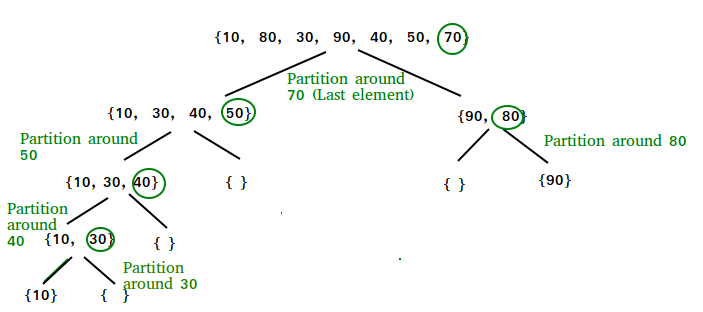
\includegraphics[scale=0.6]{QuickSort.png}
\end{center}


\end{document}






